% Options for packages loaded elsewhere
\PassOptionsToPackage{unicode}{hyperref}
\PassOptionsToPackage{hyphens}{url}
%
\documentclass[
  man]{apa6}
\usepackage{amsmath,amssymb}
\usepackage{iftex}
\ifPDFTeX
  \usepackage[T1]{fontenc}
  \usepackage[utf8]{inputenc}
  \usepackage{textcomp} % provide euro and other symbols
\else % if luatex or xetex
  \usepackage{unicode-math} % this also loads fontspec
  \defaultfontfeatures{Scale=MatchLowercase}
  \defaultfontfeatures[\rmfamily]{Ligatures=TeX,Scale=1}
\fi
\usepackage{lmodern}
\ifPDFTeX\else
  % xetex/luatex font selection
\fi
% Use upquote if available, for straight quotes in verbatim environments
\IfFileExists{upquote.sty}{\usepackage{upquote}}{}
\IfFileExists{microtype.sty}{% use microtype if available
  \usepackage[]{microtype}
  \UseMicrotypeSet[protrusion]{basicmath} % disable protrusion for tt fonts
}{}
\makeatletter
\@ifundefined{KOMAClassName}{% if non-KOMA class
  \IfFileExists{parskip.sty}{%
    \usepackage{parskip}
  }{% else
    \setlength{\parindent}{0pt}
    \setlength{\parskip}{6pt plus 2pt minus 1pt}}
}{% if KOMA class
  \KOMAoptions{parskip=half}}
\makeatother
\usepackage{xcolor}
\usepackage{graphicx}
\makeatletter
\def\maxwidth{\ifdim\Gin@nat@width>\linewidth\linewidth\else\Gin@nat@width\fi}
\def\maxheight{\ifdim\Gin@nat@height>\textheight\textheight\else\Gin@nat@height\fi}
\makeatother
% Scale images if necessary, so that they will not overflow the page
% margins by default, and it is still possible to overwrite the defaults
% using explicit options in \includegraphics[width, height, ...]{}
\setkeys{Gin}{width=\maxwidth,height=\maxheight,keepaspectratio}
% Set default figure placement to htbp
\makeatletter
\def\fps@figure{htbp}
\makeatother
\setlength{\emergencystretch}{3em} % prevent overfull lines
\providecommand{\tightlist}{%
  \setlength{\itemsep}{0pt}\setlength{\parskip}{0pt}}
\setcounter{secnumdepth}{-\maxdimen} % remove section numbering
% Make \paragraph and \subparagraph free-standing
\ifx\paragraph\undefined\else
  \let\oldparagraph\paragraph
  \renewcommand{\paragraph}[1]{\oldparagraph{#1}\mbox{}}
\fi
\ifx\subparagraph\undefined\else
  \let\oldsubparagraph\subparagraph
  \renewcommand{\subparagraph}[1]{\oldsubparagraph{#1}\mbox{}}
\fi
\newlength{\cslhangindent}
\setlength{\cslhangindent}{1.5em}
\newlength{\csllabelwidth}
\setlength{\csllabelwidth}{3em}
\newlength{\cslentryspacingunit} % times entry-spacing
\setlength{\cslentryspacingunit}{\parskip}
\newenvironment{CSLReferences}[2] % #1 hanging-ident, #2 entry spacing
 {% don't indent paragraphs
  \setlength{\parindent}{0pt}
  % turn on hanging indent if param 1 is 1
  \ifodd #1
  \let\oldpar\par
  \def\par{\hangindent=\cslhangindent\oldpar}
  \fi
  % set entry spacing
  \setlength{\parskip}{#2\cslentryspacingunit}
 }%
 {}
\usepackage{calc}
\newcommand{\CSLBlock}[1]{#1\hfill\break}
\newcommand{\CSLLeftMargin}[1]{\parbox[t]{\csllabelwidth}{#1}}
\newcommand{\CSLRightInline}[1]{\parbox[t]{\linewidth - \csllabelwidth}{#1}\break}
\newcommand{\CSLIndent}[1]{\hspace{\cslhangindent}#1}
\ifLuaTeX
\usepackage[bidi=basic]{babel}
\else
\usepackage[bidi=default]{babel}
\fi
\babelprovide[main,import]{english}
% get rid of language-specific shorthands (see #6817):
\let\LanguageShortHands\languageshorthands
\def\languageshorthands#1{}
% Manuscript styling
\usepackage{upgreek}
\captionsetup{font=singlespacing,justification=justified}

% Table formatting
\usepackage{longtable}
\usepackage{lscape}
% \usepackage[counterclockwise]{rotating}   % Landscape page setup for large tables
\usepackage{multirow}		% Table styling
\usepackage{tabularx}		% Control Column width
\usepackage[flushleft]{threeparttable}	% Allows for three part tables with a specified notes section
\usepackage{threeparttablex}            % Lets threeparttable work with longtable

% Create new environments so endfloat can handle them
% \newenvironment{ltable}
%   {\begin{landscape}\centering\begin{threeparttable}}
%   {\end{threeparttable}\end{landscape}}
\newenvironment{lltable}{\begin{landscape}\centering\begin{ThreePartTable}}{\end{ThreePartTable}\end{landscape}}

% Enables adjusting longtable caption width to table width
% Solution found at http://golatex.de/longtable-mit-caption-so-breit-wie-die-tabelle-t15767.html
\makeatletter
\newcommand\LastLTentrywidth{1em}
\newlength\longtablewidth
\setlength{\longtablewidth}{1in}
\newcommand{\getlongtablewidth}{\begingroup \ifcsname LT@\roman{LT@tables}\endcsname \global\longtablewidth=0pt \renewcommand{\LT@entry}[2]{\global\advance\longtablewidth by ##2\relax\gdef\LastLTentrywidth{##2}}\@nameuse{LT@\roman{LT@tables}} \fi \endgroup}

% \setlength{\parindent}{0.5in}
% \setlength{\parskip}{0pt plus 0pt minus 0pt}

% Overwrite redefinition of paragraph and subparagraph by the default LaTeX template
% See https://github.com/crsh/papaja/issues/292
\makeatletter
\renewcommand{\paragraph}{\@startsection{paragraph}{4}{\parindent}%
  {0\baselineskip \@plus 0.2ex \@minus 0.2ex}%
  {-1em}%
  {\normalfont\normalsize\bfseries\itshape\typesectitle}}

\renewcommand{\subparagraph}[1]{\@startsection{subparagraph}{5}{1em}%
  {0\baselineskip \@plus 0.2ex \@minus 0.2ex}%
  {-\z@\relax}%
  {\normalfont\normalsize\itshape\hspace{\parindent}{#1}\textit{\addperi}}{\relax}}
\makeatother

% \usepackage{etoolbox}
\makeatletter
\patchcmd{\HyOrg@maketitle}
  {\section{\normalfont\normalsize\abstractname}}
  {\section*{\normalfont\normalsize\abstractname}}
  {}{\typeout{Failed to patch abstract.}}
\patchcmd{\HyOrg@maketitle}
  {\section{\protect\normalfont{\@title}}}
  {\section*{\protect\normalfont{\@title}}}
  {}{\typeout{Failed to patch title.}}
\makeatother

\usepackage{xpatch}
\makeatletter
\xapptocmd\appendix
  {\xapptocmd\section
    {\addcontentsline{toc}{section}{\appendixname\ifoneappendix\else~\theappendix\fi\\: #1}}
    {}{\InnerPatchFailed}%
  }
{}{\PatchFailed}
\keywords{keywords\newline\indent Word count: X}
\DeclareDelayedFloatFlavor{ThreePartTable}{table}
\DeclareDelayedFloatFlavor{lltable}{table}
\DeclareDelayedFloatFlavor*{longtable}{table}
\makeatletter
\renewcommand{\efloat@iwrite}[1]{\immediate\expandafter\protected@write\csname efloat@post#1\endcsname{}}
\makeatother
\usepackage{csquotes}
\ifLuaTeX
  \usepackage{selnolig}  % disable illegal ligatures
\fi
\IfFileExists{bookmark.sty}{\usepackage{bookmark}}{\usepackage{hyperref}}
\IfFileExists{xurl.sty}{\usepackage{xurl}}{} % add URL line breaks if available
\urlstyle{same}
\hypersetup{
  pdftitle={Demanding resources: Converging perceptions of challenge and resource characteristics},
  pdfauthor={John Kulas1, Alicia Stachowski2, \& Renata García Prieto Palacios Roji3},
  pdflang={en-EN},
  pdfkeywords={keywords},
  hidelinks,
  pdfcreator={LaTeX via pandoc}}

\title{Demanding resources: Converging perceptions of challenge and resource characteristics}
\author{John Kulas\textsuperscript{1}, Alicia Stachowski\textsuperscript{2}, \& Renata García Prieto Palacios Roji\textsuperscript{3}}
\date{}


\shorttitle{Demanding Resources}

\authornote{

Add complete departmental affiliations for each author here. Each new line herein must be indented, like this line.

Enter author note here.

Correspondence concerning this article should be addressed to John Kulas. E-mail: \href{mailto:jtkulas@ergreports.com}{\nolinkurl{jtkulas@ergreports.com}}

}

\affiliation{\vspace{0.5cm}\textsuperscript{1} eRg\\\textsuperscript{2} University of Wisconsin - Stout\\\textsuperscript{3} PepsiCo}

\abstract{%
568 workers rated job characteristics in terms of relevance as well as perceptions as challenges, hindrances and resources. We find strong associations between characteristics such that what is viewed as a ``resource'' is also very often considered a ``challenge''. This agreement was moderated by the nature of the job characteristic.
}



\begin{document}
\maketitle

The Occupational Information Network (O*NET; onetonline.org) contains a reasonably comprehensive description of occupations (Peterson et al., 2001) which subject matter experts inform via surveys. We utilize a set of O*NET job context and activity statements contained in these surveys to explore a series of research questions about how people perceive resources, challenges, and hindrances within their jobs. There are a number of advantage to using this standard set of statements, but the primary one here lies in our ability to consider a wide range of job characteristics, with a focus on individual perceptions of each rather than limiting ourselves to a more generic set of demands or those of a limited scope.

\hypertarget{not-all-stressors-are-equal-the-challenge-hindrance-framework}{%
\subsection{Not all Stressors are Equal: The Challenge-hindrance Framework}\label{not-all-stressors-are-equal-the-challenge-hindrance-framework}}

Although the word ``stress'' often carries a negative connotation, the ``father'' of the current concept, Selye (1936), conceptualized stress much less pejoratively - rather thinking of it as a \emph{response to change}. For instance, consider the different reactions two different employees may have to being nominated to give a speech at an upcoming company event. One may appraise the nomination as a negative stressor. However, another employee may appraise the nomination to do so as an opportunity to share their experiences with more of their coworkers, or one in which they may receive recognition they have desired. Selye the physician would likely have labeled the two responses as subjective manifestations of ``distress'', and ``eustress'' (Selye, 1974). In modern I-O Psychology parlance (and more consistent with the job demands-resources model (Demerouti et al., 2001) and job demands-resources theory (Bakker \& Demerouti, 2017)), the two workers would both be characterized as appraising the speaking opportunity as a job demand, but one would be appraising the demand as a \emph{challenge} while the other would appraise the demand as a \emph{hindrance} (Cavanaugh et al., 2000). According to Cavanaugh et al. (2000), challenge demands promote mastery, personal growth, and future gains. Hindrance demands, in contrast, inhibit growth, learning and goal achievement. Perhaps not surprisingly, challenge demands are typically associated with positive outcomes, whereas hindrance demands are associated with more negative outcomes (e.g., Cavanaugh et al., 2000).

At the most broad level, we can question whether employees actually distinguish between challenges and hindrances as the theory describes. Research suggests that people can and do perceive them differently. For example, Bakker and Sanz-Vergel (2013) found that perceived work pressure can be classified as a hindrance demand, while the requirement to express emotions is a challenge demand. Webster et al. (2011) also considered three common work characteristics including workload, role ambiguity, and role conflict. Interestingly, they found that while each could be identified \emph{primarily} as a challenge or hindrance, employees could also appraise that a characteristic is simultaneously both a challenge and hindrance. However, this list of demands (workload, role ambiguity, and role conflict) is somewhat narrow. Using a very wide range of O*NET job characteristics regarding job context and activities, we explore whether challenges (positive stressors per the definition above) might actually be positively related to resources. Per the job demands-resources theory (Bakker \& Demerouti, 2017) resources are defined as physical, psychological, social, or organizational aspects of the job that may help an employee achieve work goals, reduce job demands, or promote personal growth and development (Demerouti et al., 2001). It stands to reason that a challenging demand may be considered a resource.

\emph{RQ1}: Do jobs with many resources also perceived to have many challenges?

Although we argue that the same job characteristic may be perceived as both a challenge and a resource, it is also likely that some characteristics are less likely to be viewed as mutually complementary as others. For example, a physically strenuous job requirement such as ``carrying heavy objects'' would be less likely to be viewed both as a challenge and a resource whereas a structural characteristic such as ``negotiating work schedules'' may very well be viewed (likely in different circumstances) to be both a control-oriented resource as well as a challenge. O*NET has different levels of abstraction with regard to the nature of job characteristics. We will be exploring a mid-level abstraction with seven different characteristic scales.

\emph{RQ2}: Is the association between challenge and resource characteristics moderated by type of characteristic?

\hypertarget{maybe-do-third-moderator}{%
\paragraph{Maybe do third moderator}\label{maybe-do-third-moderator}}

We also have ratings of ``\ldots the extent to which this characteristic is present in your job''. Currently we're just taking a binary yes/no approach, but it does make sense to look for moderation based on \emph{the degree to which the characteristic is present}. This is probably a better/more appropriate moderator than either of the above two\ldots{}

\hypertarget{method}{%
\section{Method}\label{method}}

We evaluate agreement across perceptions of job characteristics regarding their characterization as resource, challenge, and hindrance (Bakker \& Demerouti, 2017; Bakker et al., 2003; Demerouti et al., 2001). To capture an effectively exhaustive list of characteristics that apply to, theoretically, \emph{every} possible job, we consult the unifying framework of O*NET.

\hypertarget{participants}{%
\subsection{Participants}\label{participants}}

Eligibility requirements included being 18 or older and holding either a full- or part-time job. Participants were asked to think about their primary job while answering the survey. We sampled from a Prolific panel, resulting in 785 individuals who initially accessed the survey link. Of those, 112 indicated that they were not interested, had more than 200 missing responses, or had 20 or more identical consecutive sequential responses (Yentes \& Wilhelm, 2021). Additional screening using four embedded attention checks resulted in the retention of 568 respondents. A total of 13.57\% had been in their job less than 6 months, 19.20\% between 6 months and a year, 49.12\% between one and five years, 13.27\% between 5 and 10 years, and 4.87\% more than 10 years. Reported ages ranged from 18 to 65 with an average of 28.18 years old (SD = 7.53). Gender was captured via a free-field gender identity category, although the sample predominantly self-identified as female (52.6\%) or male (46.8\%).

\hypertarget{materials}{%
\subsection{Materials}\label{materials}}

Our survey was informed by 98 statements taken from job characteristic descriptors located within O*NET's classification of ``work activities'': 1) Information Input (5 statements), 2) Interacting with Others (17 statements), 3) Mental Processes (10 statements), and 4) Work Output (9 statements) and ``work context'' groupings: 1) Interpersonal Relationships (14 statements), 2) Physical Work Conditions (30 statements), and 3) Structural Job Characteristics (13 statements).

The O*NET descriptors are written in a similar manner to a task statement presented within a job analysis, but the level of abstraction is closer to ``responsibility'' than task. For example, the descriptor for ``level of competition'', which is an element of the ``structural job characteristics'' grouping, is \emph{How often do you have to perform public speaking in this job??} Other than minor grammatical editing (for example, changing ``the worker'' to ``you'' where applicable), we retained the O*NET wording for our item stems. We also retained O*NET's response scales, several of which were semantically unique across items, but all shared the same 5-point scale. It would likely NOT be considered controversial to referred to these as ``effectively'' Likert-type response scales.

\hypertarget{procedure}{%
\subsection{Procedure}\label{procedure}}

Respondents were recruited through Prolific. After providing consent, respondents provided ratings of whether or not each of the 98 O*NET characteristics were relevant for the respondent's primary work role. Subsequently, each respondent who agreed that an element had at least some relevance to their job was then also asked to rate that element in terms of perception of resource, challenge, and hindrance. The total number of items on the survey was less than 392 (98 characteristics x 4 administrations - the first for relevance and the remaining 3 for resources, challenges, and hindrances) because we did not ask for demand and resource evaluations for 14 O*NET characteristics that we projected would have very low frequency of endorsement across respondents (one excluded characteristic, for example, was \emph{\ldots the extent to which the worker is exposed to radiation on the job}). Furthermore, not every respondent indicated that the same characteristics were relevant to them. Therefore, each respondent had a unique set of administered items. Participants were compensated for their participation in this study in the amount of six dollars through Prolific.

\hypertarget{results}{%
\section{Results}\label{results}}

All analyses are focused on characteristics of work that were rated as being ``relevant'' to the respondents' primary job. Upon confirming that a work characteristic was relevant, respondents then also rated the extent to which that characteristic was perceived as a resources, challenge, and hindrance.

\begin{table}[tbp]

\begin{center}
\begin{threeparttable}

\caption{\label{tab:cortab}Resource, challenge, and hindrance correlations (counts data).}

\begin{tabular}{lllll}
\toprule
 & \multicolumn{1}{c}{1} & \multicolumn{1}{c}{2} & \multicolumn{1}{c}{$M$} & \multicolumn{1}{c}{$SD$}\\
\midrule
1. resource & - &  & 36.02 & 13.26\\
2. hindrance & .23*** & - & 13.09 & 13.62\\
3. challenge & .86*** & .22*** & 35.64 & 13.63\\
\bottomrule
\end{tabular}

\end{threeparttable}
\end{center}

\end{table}

\begin{figure}
\centering
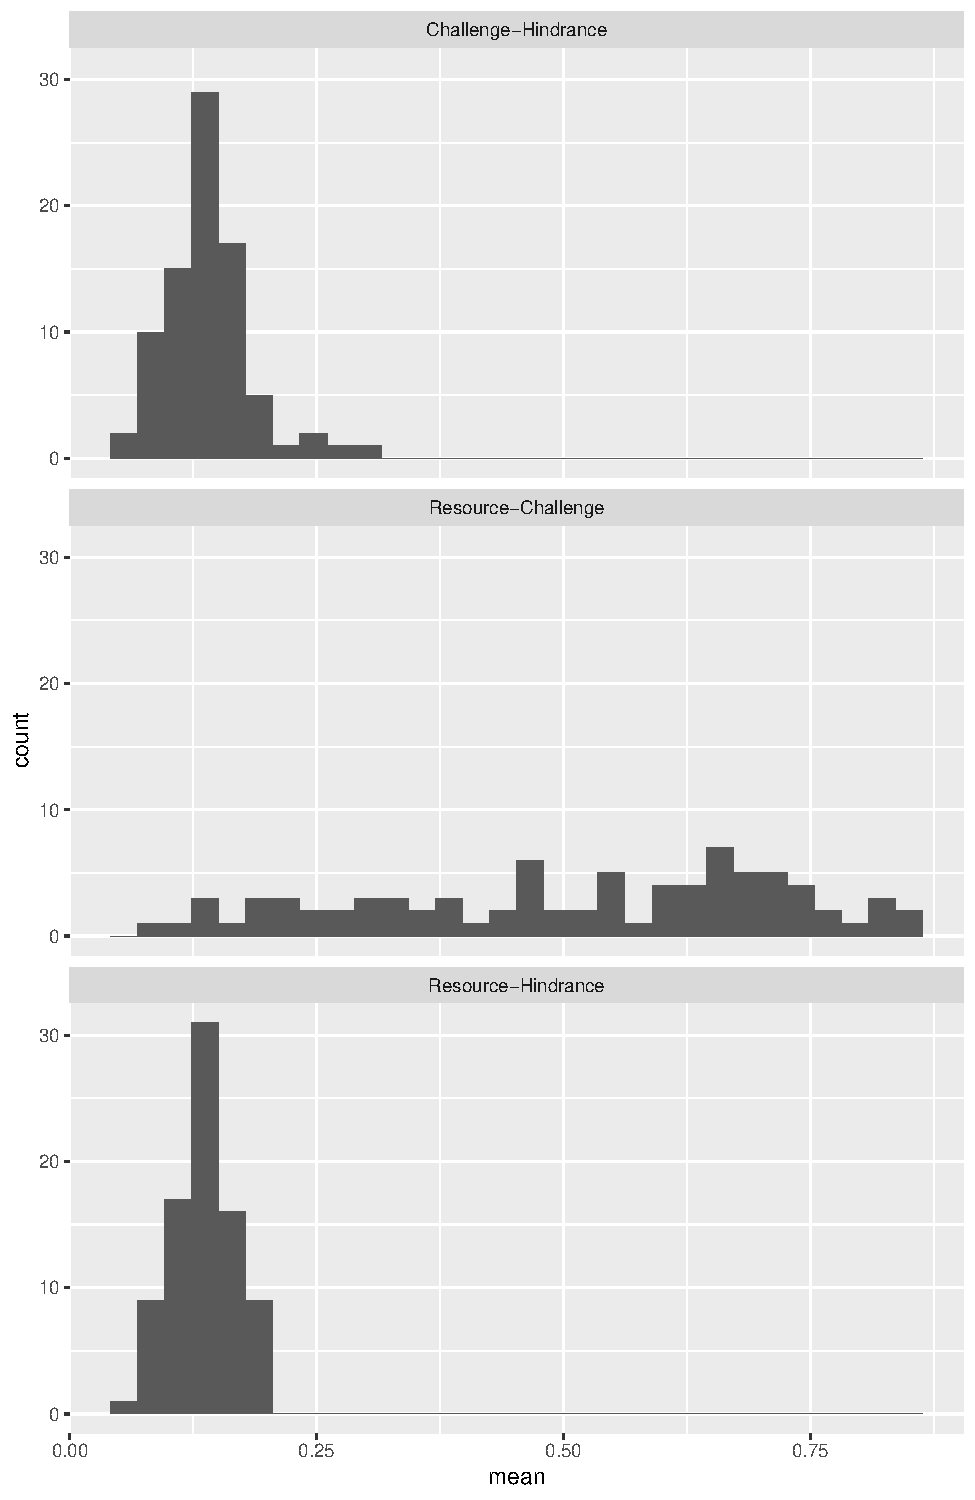
\includegraphics{SIOP2024convergence_files/figure-latex/percagree-1.pdf}
\caption{\label{fig:percagree}Percent convergence (characteristic rated consistently as, for example, both a resource and a hindrance).}
\end{figure}

\begin{figure}
\centering
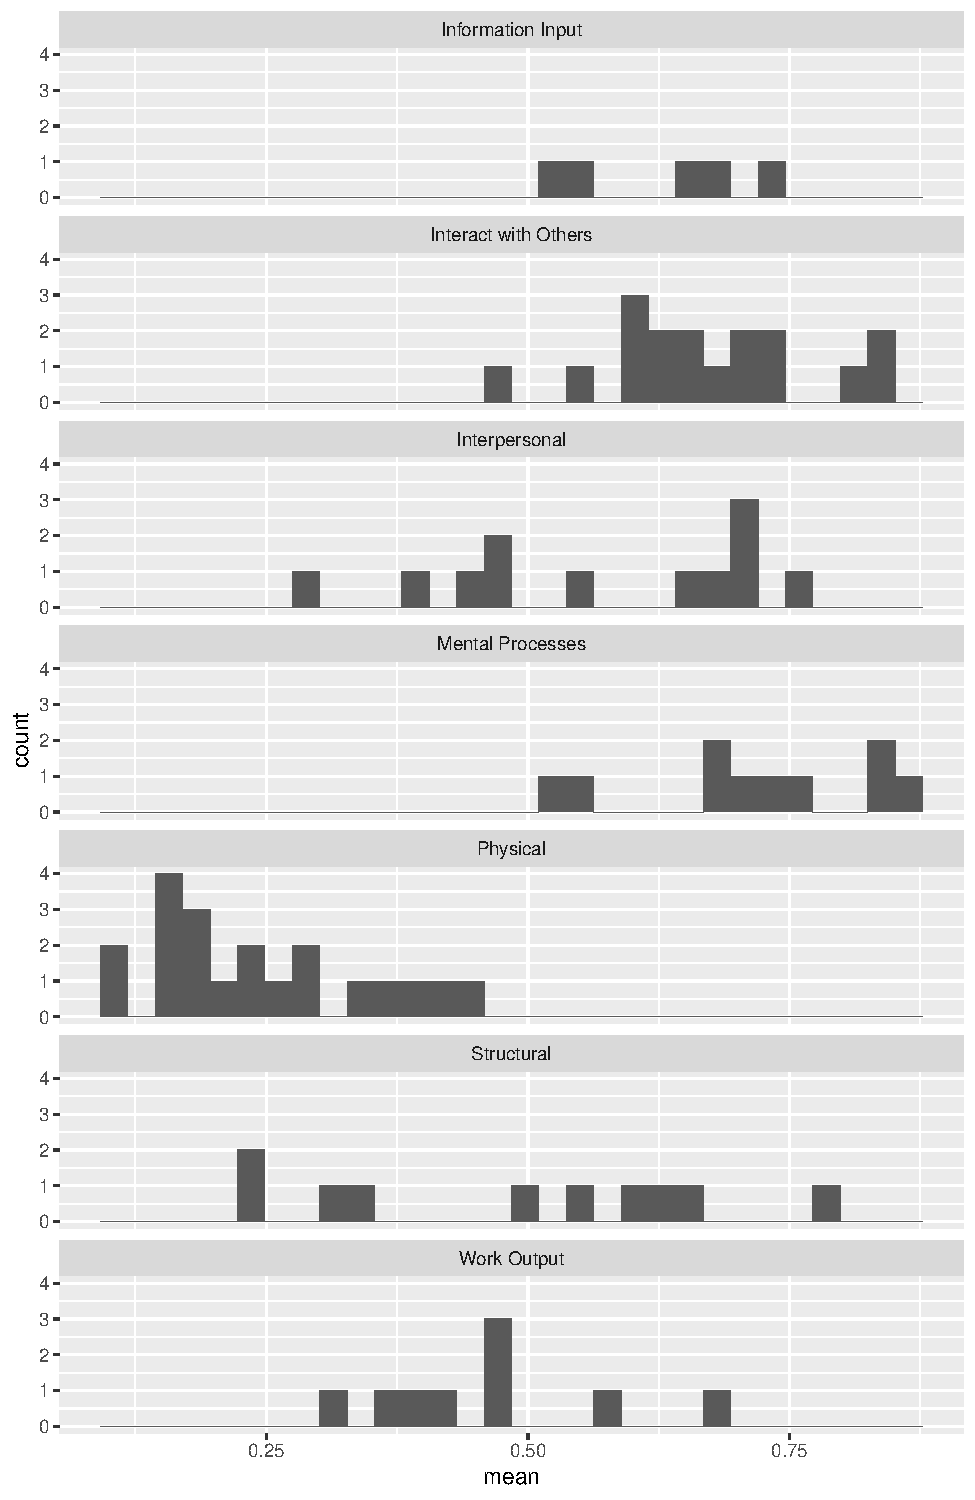
\includegraphics{SIOP2024convergence_files/figure-latex/recchall-1.pdf}
\caption{\label{fig:recchall}Resource and challenge agreement across ONet characteristic groupings (e.g., scales).}
\end{figure}

\hypertarget{resource-challenge-and-hindrance-associations}{%
\subsection{Resource, Challenge, and Hindrance Associations}\label{resource-challenge-and-hindrance-associations}}

Research Question 1 explored whether jobs with many challenges have many resources. The total number of undifferentiated challenges and resources are positively related. Table \ref{tab:cortab} shows a very high association between resources and challenges (\emph{r} = .86). These associations, however, are only capturing the relationships between these demands and resources in \emph{sheer volume}. That is, Table \ref{tab:cortab} operationalized each variable as the sheer number of resources, hindrances, or challenges that a respondent indicated were present within their job. This correlational analysis simply implies that workers who experience more resources also perceive greater challenges. The associations between resources and hindrances (\emph{r} = .23) and challenges and hindrances (\emph{r} = .22) were also significantly positive with moderate magnitude associations, suggesting that some of this ``sheer volume'' may be capturing job complexity (that is, the more complex the job, the more characteristics are relevant, and therefore the more likely it is to have \emph{more} challenges as well as \emph{more} hindrances as well as \emph{more} resources). Although we did not address job complexity as a moderator in the current paper, we do plan to do so in future investigations. Also, take note of the average numbers of resources, challenges, and hindrances cited by our sample, where these respondents generally experienced fewer hindrances in their jobs (\emph{M} = 13.09) than both resources and challenges.

\hypertarget{convergence-same-characteristic}{%
\subsection{Convergence (same characteristic)}\label{convergence-same-characteristic}}

We next looked for convergence of perception at the level of each individual job characteristic. Here, we calculated the \emph{percent of affirmative correspondence} between individual characteristic perceptions. That is, a respondent needed to agree that \emph{\ldots being in contact with others} was both a resource as well as a challenge in order to be implicated as affirmatively agreeing. We did this for each of the 84 individual characteristics that were rated as a resource, challenge, or demand and then computed an aggregate level of affirmative correspondence for each person. Figure \ref{fig:percagree} presents the results of these correspondences, showing that there was not much mutual agreement regarding characteristics being viewed as both hindrances and resources (\emph{M} = 0.14) or as challenges and hindrances (\emph{M} = 0.14). However, when a characteristic was viewed a resource, it was more likely to also be perceived as a challenge (although the correspondence also exhibited quite a bit of variability; \emph{M} = 0.51, \emph{SD} = 0.21).

\hypertarget{moderating-effects}{%
\subsubsection{Moderating effects}\label{moderating-effects}}

Figure \ref{fig:recchall} explores the possibility of moderation by \emph{type of characteristic rated} for the resource-challenge convergence. Here we categorized each characteristic by its O*NET ``scale'' (one of seven), and the graph shows greater consistency across certain characteristics (for example, \emph{Mental Processes} or \emph{Interacting with Others}) and less convergence across other \emph{types} of job activities (for example, \emph{Physical} characteristics). A repeated-measures ANOVA retaining these scales as 7 different levels of a within-subjects' independent variables yielded a treatment effect of \(F_{(6, 3,402)}\) = 613.5, \emph{p} \textless{} .001, \(\eta^2_{p}\) = 0.35 (the subjects' effect was \(F_{(567, 3402)}\) = 6.13, \emph{p} \textless{} .001. The only contrast approaching statistical significance via Tukey's HSD specification (\emph{p} = .09) was the contrast between Physical Labor (\emph{M} = 0.49) and Business and Financial Operations (\emph{M} = 0.58). Additionally, a Levene's test for homogeneity of variance was non-significant (Levene's = , \emph{p} = .

\hypertarget{discussion}{%
\section{Discussion}\label{discussion}}

The major goal of this paper was to further explore the relationships among perceptions of job characteristics as challenge demands, hindrance demands, and resources. Our findings perhaps most notably highlight the importance of dissociating the \emph{nature} of job demands.

IMPLICATION: Distinguishing between different kinds of work demands has implications for not only the employees themselves, but also teams they may be a part of, managers and the like. This is because demands appraised as a challenge promote mastery, personal growth, and future gains. Those appraised as a hindrance, in contrast, inhibit growth, learning and goal achievement. Perhaps not surprisingly, challenge demands are typically associated with positive outcomes, whereas hindrance demands are associated with more negative outcomes (e.g., Cavanaugh et al., 2000).

Similar to the eustress/distress distinction (e.g., Selye, 1974), it would seem as though demands should perhaps be thought of in a valenced manner (e.g., is it a ``good'' demand or a ``bad'' demand). We did not probe for dependent variable associations, however, Cavanaugh et al. (2000) found that challenge demands were positively related to job satisfaction and negatively related to job search behaviors, while hindrance demands demonstrated the opposite patterns in a sample of managers. We also have some evidence that challenge-hindrance appraisals are related to engagement in the expected direction whereby hindrance appraisals are negatively associated with engagement and challenge appraisals are positively associated with engagement (Crawford et al. (2010)). Podsakoff et al. (2007)'s meta-analysis also found that challenge demands were positively related to job satisfaction and organizational commitment and negatively related to both turnover intentions and actual turnover, while hindrance demands again produced the opposite patterns of relationship. Although we did not probe for outcome associations, the current study does suggest that hindrance demands also operate in a manner different than challenge demands with regard to their association with resource appraisals.

In terms of convergence of resource and challenge appraisals, there was quite a bit of variability (e.g., Figure \ref{fig:percagree}), but that variability was partially explained by the nature of the characteristic being evaluated (e.g., Figure \ref{fig:recchall}). Physical job characteristics such as, for example, the amount of ``time spent bending or twisting the body'' may be much more likely to be appraised as a challenging demand (but not a resource). Other \emph{types} of job requirements, however, such as a mental process like, ``scheduling work and activities'' might reasonably be expected to exhibit greater convergence. We suspect that there are other moderators that help explain this association/ disassociation between challenges and resources, and would like to incorporate variables such as a respondents' personality in future investigations.

\hypertarget{references}{%
\section*{References}\label{references}}
\addcontentsline{toc}{section}{References}

\hypertarget{refs}{}
\begin{CSLReferences}{1}{0}
\leavevmode\vadjust pre{\hypertarget{ref-bakker2017job}{}}%
Bakker, A. B., \& Demerouti, E. (2017). Job demands--resources theory: Taking stock and looking forward. \emph{Journal of Occupational Health Psychology}, \emph{22}(3), 273.

\leavevmode\vadjust pre{\hypertarget{ref-bakker2013weekly}{}}%
Bakker, A. B., \& Sanz-Vergel, A. I. (2013). Weekly work engagement and flourishing: The role of hindrance and challenge job demands. \emph{Journal of Vocational Behavior}, \emph{83}(3), 397--409.

\leavevmode\vadjust pre{\hypertarget{ref-cavanaugh2000empirical}{}}%
Cavanaugh, M. A., Boswell, W. R., Roehling, M. V., \& Boudreau, J. W. (2000). An empirical examination of self-reported work stress among US managers. \emph{Journal of Applied Psychology}, \emph{85}(1), 65.

\leavevmode\vadjust pre{\hypertarget{ref-crawford2010linking}{}}%
Crawford, E. R., LePine, J. A., \& Rich, B. L. (2010). Linking job demands and resources to employee engagement and burnout: A theoretical extension and meta-analytic test. \emph{Journal of Applied Psychology}, \emph{95}(5), 834.

\leavevmode\vadjust pre{\hypertarget{ref-demerouti2001job}{}}%
Demerouti, E., Bakker, A. B., Nachreiner, F., \& Schaufeli, W. B. (2001). The job demands-resources model of burnout. \emph{Journal of Applied Psychology}, \emph{86}(3), 499.

\leavevmode\vadjust pre{\hypertarget{ref-peterson2001understanding}{}}%
Peterson, N. G., Mumford, M. D., Borman, W. C., Jeanneret, P. R., Fleishman, E. A., Levin, K. Y., Campion, M. A., Mayfield, M. S., Morgeson, F. P., Pearlman, K., et al. (2001). Understanding work using the occupational information network (o* NET): Implications for practice and research. \emph{Personnel Psychology}, \emph{54}(2), 451--492.

\leavevmode\vadjust pre{\hypertarget{ref-podsakoff2007differential}{}}%
Podsakoff, N. P., LePine, J. A., \& LePine, M. A. (2007). Differential challenge stressor-hindrance stressor relationships with job attitudes, turnover intentions, turnover, and withdrawal behavior: A meta-analysis. \emph{Journal of Applied Psychology}, \emph{92}(2), 438.

\leavevmode\vadjust pre{\hypertarget{ref-selye1936syndrome}{}}%
Selye, H. (1936). A syndrome produced by diverse nocuous agents. \emph{Nature}, \emph{138}(3479), 32--32.

\leavevmode\vadjust pre{\hypertarget{ref-selye1974stress}{}}%
Selye, H. (1974). \emph{Stress without distress}. Lippincott Williams \& Wilkins.

\leavevmode\vadjust pre{\hypertarget{ref-webster2011extending}{}}%
Webster, J. R., Beehr, T. A., \& Love, K. (2011). Extending the challenge-hindrance model of occupational stress: The role of appraisal. \emph{Journal of Vocational Behavior}, \emph{79}(2), 505--516.

\end{CSLReferences}


\end{document}
